\documentclass{beamer}

\hypersetup{pdfpagemode=FullScreen}

\usepackage[utf8]{inputenc}
\usepackage{default}
\usepackage[italian]{babel}
\usepackage{amsmath}
\usepackage{amsfonts}
\usepackage{xfrac}
\usepackage{tabularx}

\usepackage{graphicx}
\graphicspath{{img/}}

\newcommand{\der}[2]{\frac{\partial #1}{\partial #2}}
\newcommand{\dder}[2]{\frac{\partial^2 #1}{\partial #2^2}}
\newcommand{\dmix}[3]{\frac{\partial^2 #1}{\partial #2 \partial #3}}

\AtBeginSection[]
{
  \begin{frame}
    \frametitle{Table of Contents}
    \tableofcontents[currentsection]
  \end{frame}
}

%%presentation theme
\usetheme{Warsaw}

%%remove navigation symbols
\beamertemplatenavigationsymbolsempty

%%add page numbering
\useoutertheme{infolines}
% \setbeamertemplate{footline}

\begin{document}


%%%%%%%%%%%%%%%%%%%%%%%%%%%%%%%%%%%%%%%%%%%%%%%%%%%%%%%%%%%%%%%%%%%%%%%%%%%%%%%%%%%%%%%%%%%%%%%%%%%%%%%%%%%%%%%%%%%%%%%%%%%%%%%%%%%%%%%%%%%%%%%%%%%%%%%%%%%%%%%%%%%%%%%%%%%%%%%%%%%%%%%%%%%%%%%%%%%%%%%%%%%%%%%%%%%%%%%%%%%%%%%%%%%%%%%%%%%%%%%%%%%%%%%%%%%%%%%%%%
\section{Introduzione}
\begin{frame}
\frametitle{Il progetto}
\begin{block}{Scopo}
Lo scopo è di creare una piccola libreria per il pricing di derivati finanziari con il metodo degli elementi finiti, appoggiandosi sulla libreria \textsf{deal.ii}.
L'idea è che l'utilizzatore possa sia utilizzare gli oggetti presenti, sia crearne altri con grande facilità nel caso ne avesse bisogno.
\end{block}
\pause
\begin{block}{Motivazioni}
La procedura pi\`u diffusa in finanza è di usare le differenze finite. Gli elementi finiti, a fronte di una maggiore difficoltà implementativa, risultano essere più vantaggiosi.
\end{block}
\end{frame}

%%%%%%%%%%%%%%%%%%%%%%%%%%%%%%%%%%%%%%%%%%%%%%%%%%%%%%%%%%%%%%%%%%%%%%%%%%%%%%%%%%%%%%%%%%%%%%%%%%%%%%%%%%%%%%%%%%%%%%%%%%%%%%%%%%%%%%%%%%%%%%%%%%%%%%%%%%%%%%%%%%%%%%%%%%%%%%%%%%%%%%%%%%%%%%%%%%%%%%%%%%%%%%%%%%%%%%%%%%%%%%%%%%%%%%%%%%%%%%%%%%%%%%%%%%%%%%%%%%
\section{Il problema}

\begin{frame}[t]
\frametitle{L'equazione da risolvere}
\begin{overlayarea}{\linewidth}{3cm}
\only<-5>{\begin{multline*}
\alert<2>{\der{C}{t}+\frac{\sigma^2}{2}S^2\dder{C}{S}+rS\der{C}{S}-rC}+\\ + 
\alert<3>{\int_\mathbb{R}\left(C(t,Se^y)\alert<4>{-C(t,S)-S(e^y-1)\der{C}{S}(t,S)}\right)\nu(dy)}=0
\end{multline*}}

\only<6>{\begin{multline*}
\der{u}{t}+\left(r-\frac{\sigma^2}{2}\right)\der{u}{x}+\frac{\sigma^2}{2}\dder{u}{x}-ru\\
+\int_\mathbb{R}\left( u(t,x+y)-u(t,x)-(e^y-1)\der{u}{x}\right)\nu(dy)=0
\end{multline*}}
\end{overlayarea}
con opportune condizioni al contorno.\\
\pause
Possiamo scomporre il problema in due parti
\begin{itemize}[<+->]
\item La parte differenziale, trattata in modo usuale con l'aiuto della libreria \textsf{deal.ii}
\item La parte integrale, che necessita di un trattamento speciale. \only<4>{Separabile in due pezzi.}
\end{itemize}
\pause
Trasformazioni \alert<5>{\emph{price}} e \alert<6>{\emph{logprice}}
\end{frame}

%%%%%%%%%%%%%%%%%%%%%%%%%%%%%%%%%%%%%%%%%%%%%%%%%%%%%%%%%%%%%%%%%%%%%%%%%%%%%%%%%%%%%%%%%%%%%%%%%%%%%%%%%%%%%%%%%%%%%%%%%%%%%%%%
\begin{frame}
 \frametitle{Scomposizione della parte integrale}
\only<1>{
Definendo nel modo seguente le quantità
 \begin{align*}
 \hat{\alpha}&=\int_\mathbb{R}(e^y-1)\nu(y)dy \\
 \hat{\lambda}&=\int_\mathbb{R}\nu(y)dy
\end{align*}
l'equazione diventa
\begin{equation*}
\der{C}{t}+\frac{\sigma^2}{2}S^2\dder{C}{S}+(r-\hat{\alpha})S\der{C}{S}-(r+\hat{\lambda})C+ \int_\mathbb{R}C(t,Se^y)\nu(y)dy=0
\end{equation*}
}
\only<2>{
Analogamente per la trasformazione logprice si ha
\begin{align*}
\hat{\lambda}&=\int_{\mathbb{R}}\nu(y)dy,\\
\hat{\alpha}&=\int_{\mathbb{R}}(e^y-1)\nu(y)dy,
\end{align*}
con rispettiva equazione
\begin{equation*}
\der{u}{t}+\left(r-\frac{\sigma^2}{2}-\hat{\alpha}\right)\der{u}{x}+\frac{\sigma^2}{2}\dder{u}{x}-(r+\hat{\lambda})u+\int_\mathbb{R}u(t,x+y)\nu(y)dy=0
\end{equation*}
}
\end{frame}


%%%%%%%%%%%%%%%%%%%%%%%%%%%%%%%%%%%%%%%%%%%%%%%%%%%%%%%%%%%%%%%%%%%%%%%%%%%%%%%%%%%%%%%%%%%%%%%%%%%%%%%%%%%%%%%%%%%%%%%%%%%%%%%%
\begin{frame}
\frametitle{In due dimensioni}
\only<1>{
Con la trasformazione \emph{Price}
\begin{multline*}
 \der{C}{t}+(r-\hat{\alpha}_1)S_1\der{C}{S_1}+(r-\hat{\alpha}_2)S_2\der{C}{S_2}+\frac{\sigma^2_1}{2}S_1^2\dder{C}{S_1}+\frac{\sigma^2_2}{2}S_2^2\dder{C}{S_2}\\
 +\rho\sigma_1\sigma_2S_1S_2\dmix{C}{S_1}{S_2}-(r+\lambda_1+\lambda_2)C\\
 +\int_\mathbb{R}C(t,S_1e^y,S_2)\nu_1(y)dy+\int_\mathbb{R}C(t,S_1,S_2e^y)\nu_2(y)dy=0
\end{multline*}
}

\only<2>{
Con la trasformazione \emph {Logprice}
\begin{multline*}
\der{u}{t}+\frac{\sigma_1^2}{2}\dder{u}{x_1}+\frac{\sigma_2^2}{2}\dder{u}{x_2}+\rho\sigma_1\sigma_2\dmix{u}{x_1}{x_2}+
\left(r-\frac{\sigma_1^2}{2}-\hat{\alpha_1}\right)\der{u}{x_1}\\+
\left(r-\frac{\sigma_2^2}{2}-\hat{\alpha_2}\right)\der{u}{x_2}-(r+\hat{\lambda_1}+\hat{\lambda_2})u\\+
\int_\mathbb{R}u(t,x_1+y,x_2)\nu_1(y)dy+
\int_\mathbb{R}u(t,x_1,x_2+y)\nu_2(y)dy=0
\end{multline*}
}

\end{frame}



%%%%%%%%%%%%%%%%%%%%%%%%%%%%%%%%%%%%%%%%%%%%%%%%%%%%%%%%%%%%%%%%%%%%%%%%%%%%%%%%%%%%%%%%%%%%%%%%%%%%%%%%%%%%%%%%%%%%%%%%%%%%%%%%

\begin{frame}[t]
 \frametitle{Discretizzazione}
 \begin{overprint}
 Data una griglia con nodi $S_i$
\end{overprint}
\only<1-3>{\begin{itemize}
  \item<1-3> Per la parte differenziale, si scrive la formulazione variazionale e la si discetizza nel modo usuale 
  
  \item<2,3> Per la parte integrale, si calcola il valore della parte integrale relativa al nodo $S_i$
  \begin{equation*}
   J^1(S_i)=\int_\mathbb{R}C(t,S_1e^y,S_2)\nu_1(y)dy
  \end{equation*}
	ottenendo una vettore $\mathbf{J}$ funzione di $S_i$. Tale funzione va poi scritta come elemento dello spazio a elementi finiti 
	
	\item<3> Per la discretizzazione temporale, viene applicato uno schema di eulero implicito, ma la parte integrale viene lasciata esplicita. Lo schema è stabile se Stabile se $\frac{1}{dt}<\lambda$.
	 \end{itemize}}
\only<4>{
\begin{block}{}
Otteniamo dunque il seguente schema, con $\mathbf{C}_h^k$ vettore componenti soluzione al tempo $k$
\begin{equation*}
 M_1\mathbf{C}_h^k=M_2\mathbf{C}_h^{k+1}+M\mathbf{J}^1+M\mathbf{J}^2
\end{equation*}
\end{block}}
\end{frame}




%%%%%%%%%%%%%%%%%%%%%%%%%%%%%%%%%%%%%%%%%%%%%%%%%%%%%%%%%%%%%%%%%%%%%%%%%%%%%%%%%%%%%%%%%%%%%%%%%%%%%%%%%%%%%%%%%%%%%%%%%%%%%%%%


\begin{frame}
 \frametitle{Calcolo dell'integrale in forma \emph{Price}}
\begin{columns}[C]
%%explanation column
\only<1>{
\begin{column}[t]{.5\linewidth}

Ricordiamo l'integrale da calcolare

\begin{equation*}
 \int_\mathbb{R}C(t,Se^y)\nu(y)dy
\end{equation*}
al quale applichiamo il cambio di variabile
\begin{equation*}
 z=Se^y
\end{equation*}
\end{column}
}

\only<2->{
\begin{column}[t]{.5\linewidth}

L'integrale diventa allora 
\begin{equation*}
\int_0^\infty \frac{C(t,z)}{z}\nu\left(\log\left(\frac{z}{S}\right)\right)dz
\end{equation*}

\only<3->{
Quindi per ogni cella, si calcolano i contributi dovuti alla cella
}

\only<4->{
e si distribuiscono ai nodi di competenza:
\begin{itemize}
 \item In 1d, a tutti i nodi.
 \item In 2d, solo a quelli che giaciono sulla retta passante per la faccia selezionata. \only<4>{Prima sull'asse x.} \only<5>{Poi sull'asse y.}
\end{itemize}
}
\end{column}
}

%%image column
\begin{column}[t]{.5\linewidth}

\only<-2>{
\begin{figure}
\centering
\includegraphics[width=\linewidth,clip=true,trim=0 0 0 100]{BaseGrid}
\caption{Una semplice griglia strutturata}
\end{figure}}

\only<3>{
\begin{figure}
\centering
\includegraphics[width=\linewidth,clip=true,trim=0 0 0 100]{CellSelected}
\caption{Poniamoci su una cella}
\end{figure}}

\only<4>{
\begin{figure}
\centering
\includegraphics[width=\linewidth,clip=true,trim=0 0 0 100]{Integrating_on_x}
\caption{I contributi della cella ai nodi x}
\end{figure}}

\only<5>{
\begin{figure}
\centering
\includegraphics[width=\linewidth,clip=true,trim=0 0 0 100]{Integrating_on_y}
\caption{I contributi della cella ai nodi y}
\end{figure}}

\end{column}
\end{columns}
\end{frame}

%%%%%%%%%%%%%%%%%%%%%%%%%%%%%%%%%%%%%%%%%%%%%%%%%%%%%%%%%%%%%%%%%%%%%%%%%%%%%%%%%%%%%%%%%%%%%%%%%%%%%%%%%%%%%%%%%%%%%%%%%%%%%%%%

\begin{frame}
 \frametitle{Calcolo dell'integrale in forma \emph{logprice}}
 \begin{columns}[C]
%%explanation column
\only<1->{
\begin{column}[t]{.5\linewidth}


In questo caso l'integrale da calcolare è

\begin{equation*}
 \int_{-\infty}^\infty u(t,x+y)\nu(y)dy
\end{equation*}
su una griglia qualunque. Notare come si può uscire dal domininio a causa del termine $x+y$\\

\only<2->{
In questo caso si cicla su tutti i vertici. Selezionato un vertice $i$,}
\only<3->{
si avranno dei nodi di quadratura in direzione $x$ e si quadra su $x_i+z_l$ (in blu), e se la dimensione è due, anche su $y$ lungo $y_i+z_l$.} 
\end{column}
}

%%image column
\begin{column}[t]{.5\linewidth}

\only<1>{
\begin{figure}
\centering
\includegraphics[width=\linewidth,clip=true,trim=0 0 0 100]{BaseGrid}
\caption{Una griglia}
\end{figure}}

\only<2>{
\begin{figure}
\centering
\includegraphics[width=\linewidth,clip=true,trim=0 0 0 100]{VertexSelected}
\caption{Poniamoci su un nodo}
\end{figure}}

\only<3->{
\begin{figure}
\centering
\includegraphics[width=\linewidth,clip=true,trim=0 0 0 100]{LogPrice_X_and_Y_integr}
\caption{Calcolo lungo le direzioni}
\end{figure}}

\end{column}
\end{columns}
 
\end{frame}

%%%%%%%%%%%%%%%%%%%%%%%%%%%%%%%%%%%%%%%%%%%%%%%%%%%%%%%%%%%%%%%%%%%%%%%%%%%%%%%%%%%%%%%%%%%%%%%%%%%%%%%%%%%%%%%%%%%%%%%%%%%%%%%%%%%%%%%%%%%%%%%%%%%%%%%%%%%%%%%%%%%%%%%%%%%%%%%%%%%%%%%%%%%%%%%%%%%%%%%%%%%%%%%%%%%%%%%%%%%%%%%%%%%%%%%%%%%%%%%%%%%%%%%%%%%%%%%%
\section{Struttura del codice}

\begin{frame}
\frametitle{La libreria \textsf{deal.ii}}
\begin{block}{Libreria \textsf{deal.ii}}
Una potente libreria opensource ad elementi finiti sui quadrilateri. Molto completa e semplice da utilizzare all'inizio, permette di risolvere problemi variazionali fino a 3 dimensioni con poche righe di codice. 
\end{block}

\pause
\begin{block}{Vantaggi}
 \begin{itemize}
  \item Documentazione molto ampia e chiara, a cui si aggiunge la presenza di 51 tutorial programs che illustrano come usare la libreria per problemi tipici
  \item Organizzata in moduli che coprono le diverse aree di un problema ad elementi finiti (\emph{creazione griglie, algebra lineare, output risultati, etc})
 \end{itemize}
\end{block}
\end{frame}
%%%%%%%%%%%%%%%%%%%%%%%%%%%%%%%%%%%%%%%%%%%%%%%%%%%%%%%%%%%%%%%%%%%%%%%%%%%%%%%%%%%%%%%%%%%%%%%%%%%%%%%%%%%%%%%%%%%%%%%%%%%%%%%%%

\begin{frame}
\frametitle{La nostra implementazione }
 Tre strutture chiave per il problema
 \begin{block}{Classi Opzione}
Rappresentano il problema e gestiscono creazione griglia, assemblaggio sistema e soluzione.
 \end{block}
 \begin{block}{Classi Model}
 I vari modelli utilizzati in finanza sono rappresentati con questa classe, la cui interfaccia è stabilita da una classe base astratta.
 \end{block}
 \begin{block}{Classi Integrali}
  Il calcolo della parte integrale è gestito da queste classi, e le Opzioni salvano un puntatore a un oggetto di questo tipo. 
 \end{block}
 Tutte sfruttanti il meccanismo dell'ereditarietà al fine di COMPLETE HERE
\end{frame}

%%%%%%%%%%%%%%%%%%%%%%%%%%%%%%%%%%%%%%%%%%%%%%%%%%%%%%%%%%%%%%%%%%%%%%%%%%%%%%%%%%%%%%%%%%%%%%%%%%%%%%%%%%%%%%%%%%%%%%%%%%%%%%%%%

\begin{frame}[t]
 \frametitle{Le classi Opzione}

 Seguendo la linea di \textsf{deal.ii}, le classi opzione costituiscono il \emph{core} del programma ad elementi finiti. Implementano i vari metodi necessari per la soluzione del problema.\\ Le classi foglia sono quelle effettivamente usate, in quanto implementano tutti i metodi.
 \only<1>{\begin{figure}
  \centering
  \includegraphics[width=\linewidth]{classOptionBase}
 \caption{Schema delle classi Opzione}
 \end{figure}}
 \only<2->{
 \begin{block}{Factory di Opzioni}
  Per facilitare la creazione di opzioni all'utente, è stata creata una \emph{Factory} che permette di creare i vari oggetti \textbf{Opzione} con un'interfaccia comune.
 \end{block}
 }
 \only<3->{
 \begin{block}{Estensibile}
  L'utente pu\`o sia utilizzare le opzioni gi\`a esistenti, che crearne delle nuove partendo dal secondo o dal terzo livello di ereditarietà.
 \end{block}
}
\end{frame}


%%%%%%%%%%%%%%%%%%%%%%%%%%%%%%%%%%%%%%%%%%%%%%%%%%%%%%%%%%%%%%%%%%%%%%%%%%%%%%%%%%%%%%%%%%%%%%%%%%%%%%%%%%%%%%%%%%%%%%%%%%%%%%%%%
\iffalse
\begin{frame}
 \frametitle{Le classi Model}
 
\end{frame}
\fi
%%%%%%%%%%%%%%%%%%%%%%%%%%%%%%%%%%%%%%%%%%%%%%%%%%%%%%%%%%%%%%%%%%%%%%%%%%%%%%%%%%%%%%%%%%%%%%%%%%%%%%%%%%%%%%%%%%%%%%%%%%%%%%%%%
\begin{frame}[t]
 \frametitle{Le classi Integrale}
 Per calcolare la parte integrale, sono state create una serie di classi. Il secondo livello di ereditarietà distingue fra \emph{price} e \emph{logprice}, mentre le classi foglia implementano quadrature specifiche ai modelli.

 \begin{figure}
  \centering
  \includegraphics[width=\linewidth]{classLevyIntegralBase}
 \caption{Schema delle classi LevyIntegral}
 \end{figure}
 \pause
 \begin{block}{anything else?}

 \end{block}
\end{frame}

%%%%%%%%%%%%%%%%%%%%%%%%%%%%%%%%%%%%%%%%%%%%%%%%%%%%%%%%%%%%%%%%%%%%%%%%%%%%%%%%%%%%%%%%%%%%%%%%%%%%%%%%%%%%%%%%%%%%%%%%%%%%%%%%%%%%%%%%%%%%%%%%%%%%%%%%%%%%%%%%%%%%%%%%%%%%%%%%%%%%%%%%%%%%%%%%%%%%%%%%%%%%%%%%%%%%%%%%%%%%%%%%%%%%%%%%%%%%%%%%%%%%%%%%%%%%%%%%%%
\section{Risultati}

\begin{frame}[t]
 \frametitle{\emph{Price} v.s \emph{LogPrice}}
Con entrambi i metodi si ottengono risultati corretti e soddisfacenti:

%spazio fra le righe!  
\renewcommand{\arraystretch}{1.5}

\only<1>{
\begin{table}
\centering
\begin{tabular}{|p{0.43\linewidth}|p{0.43\linewidth}|}
\hline
\emph{Price} & \emph{LogPrice}\\
\hline
In 1d molto veloce & In 1d mediamente veloce\\
In 2d buone performance & In 2d lento \\
Non parallelizzabile & Parallelizzabile, quindi più veloce di \emph{Price} 1d \\
No \emph{mesh adapting} in 2d & \emph{Mesh adapting} anche in 2d, migliorando le performance\\
Troncamento del domionio può introdurre problemi & Nessun problema troncamento dominio \\
\hline
\end{tabular}
\caption{Confronto fra \emph{Price} e \emph{LogPrice}}
\end{table}}

\only<2>{
\begin{figure}
 \centering
 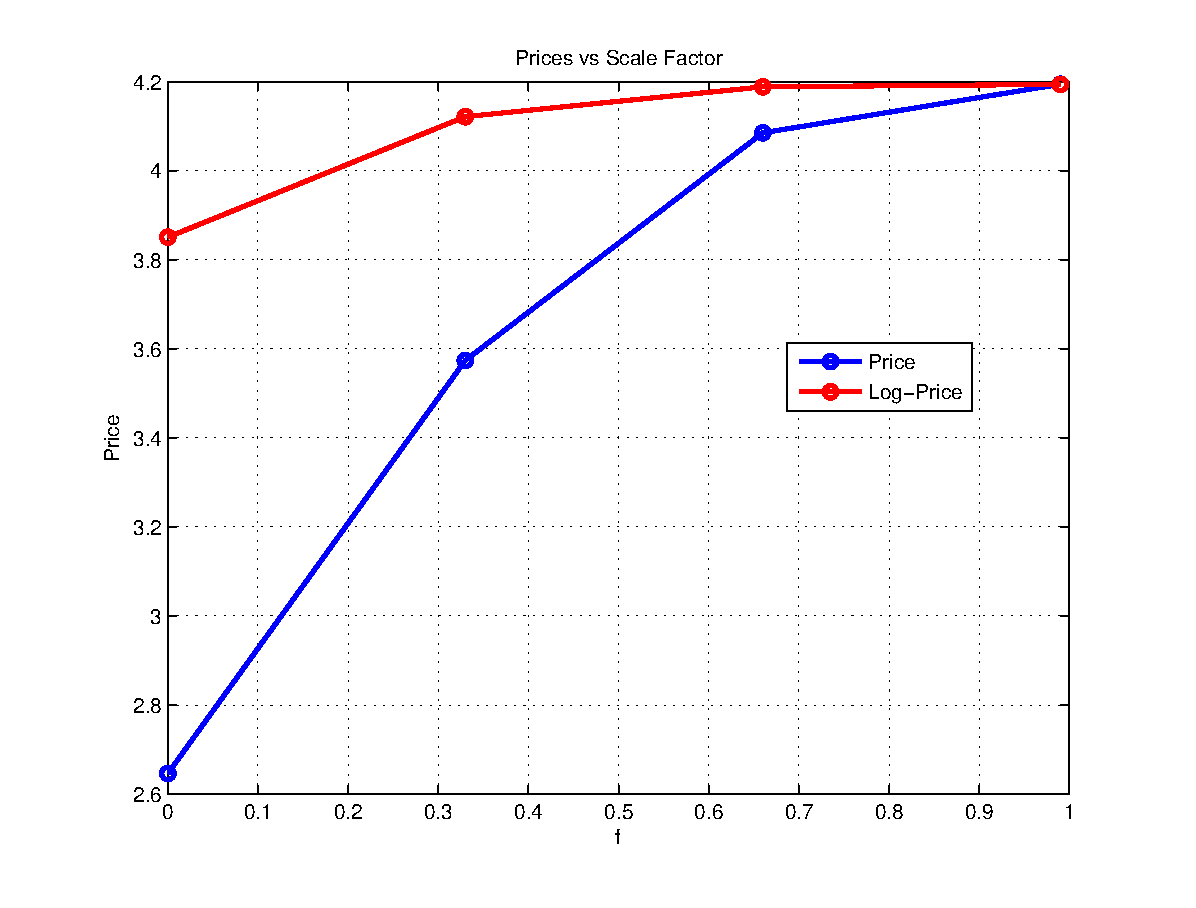
\includegraphics[width=\textwidth,height=0.7\textheight,keepaspectratio]{test2-scalefactor}
\caption{Convergenza del prezzo per una put al variare dello \emph{scaling factor}}
 \end{figure}
}
\end{frame}

%%%%%%%%%%%%%%%%%%%%%%%%%%%%%%%%%%%%%%%%%%%%%%%%%%%%%%%%%%%%%%%%%%%%%%%%%%%%%%%%%%%%%%%%%%%%%%%%%%%%%%%%%%%%%%%%%%%%%%%%%%%%%%%%

\begin{frame}
 \frametitle{}
\end{frame}


%%%%%%%%%%%%%%%%%%%%%%%%%%%%%%%%%%%%%%%%%%%%%%%%%%%%%%%%%%%%%%%%%%%%%%%%%%%%%%%%%%%%%%%%%%%%%%%%%%%%%%%%%%%%%%%%%%%%%%%%%%%%%%%%%%%%%%%%%%%%%%%%%%%%%%%%%%%%%%%%%%%%%%%%%%%%%%%%%%%%%%%%%%%%%%%%%%%%%%%%%%%%%%%%%%%%%%%%%%%%%%%%%%%%%%%%%%%%%%%%%%%%%%%%%%%%%%%%%%
\section{Conclusioni}

\end{document}